%%%%%%%%%%%%%%%%%%%%%%%%%%%%%%%%%%%%%%%%%%%%%%%%%%%%%%%%%%%
% --------------------------------------------------------
% Tau
% LaTeX Template
% Version 2.4.4 (28/02/2025)
%
% Author: 
% Guillermo Jimenez (memo.notess1@gmail.com)
% 
% License:
% Creative Commons CC BY 4.0
% --------------------------------------------------------
%%%%%%%%%%%%%%%%%%%%%%%%%%%%%%%%%%%%%%%%%%%%%%%%%%%%%%%%%%%

\documentclass[9pt,a4paper,column,twoside]{tau-class/tau}
\usepackage[english]{babel}
\usepackage{booktabs}


%% Spanish babel recomendation
% \usepackage[spanish,es-nodecimaldot,es-noindentfirst]{babel} 

%% Draft watermark
% \usepackage{draftwatermark}

%----------------------------------------------------------
% TITLE
%----------------------------------------------------------

\journalname{Intro Microelectronic Circuits with Laboratory}
\title{MOS Transistor Characteristics and Simple MOS Current Mirrors}

%----------------------------------------------------------
% AUTHORS, AFFILIATIONS AND PROFESSOR
%----------------------------------------------------------

\author[1]{Elias Tuthill}
\author[1]{Henry Tejada Deras}
\author[1]{Anika Mahesh}

%----------------------------------------------------------

\affil[1]{Franklin W. Olin College of Engineering}

%----------------------------------------------------------
% FOOTER INFORMATION
%----------------------------------------------------------

\institution{Franklin W. Olin College of Engineering}
\footinfo{Intro Microelectronic Circuits with Laboratory}
\theday{March 23, 2026}
\leadauthor{Tuthill et. al.}

%----------------------------------------------------------

\begin{document}
		
    \maketitle 
    \thispagestyle{firststyle} 
    % \tauabstract 
    % \tableofcontents
    % \linenumbers 
    
%----------------------------------------------------------

\section{Input/Gate Characteristics}
	\subsection{Results}

	\begin{figure}[H]
 		\centering
   		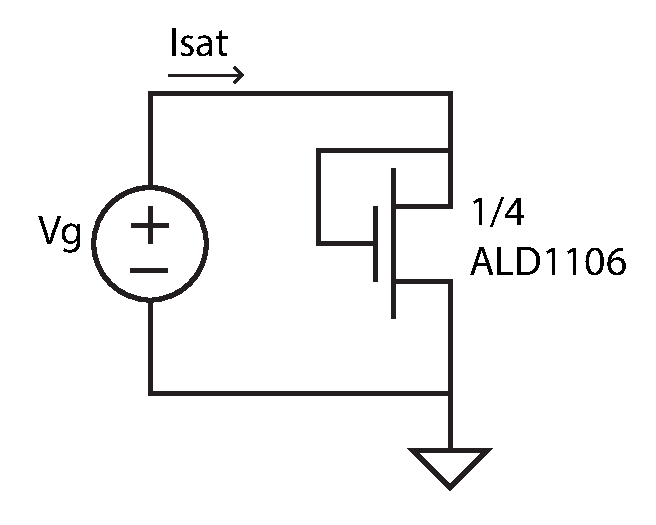
\includegraphics[width=0.6\linewidth]{../diagrams/lab4_exp1_circuit.pdf}
   		\caption{The schematic for the experimental setups used in Experiment 1. Each of the four ALD1106 transistors were used.}\label{fig:exp1_diag}
	\end{figure}
	\begin{table}[h]
		\centering
		\begin{tabular}{c c c c}
		\toprule
		MOSFET & $I_s$ (A) & $\kappa$ & $V_{T0}$ (V) \\
		\midrule
		1 & $1.6941\times10^{-6}$ & 0.7365 & 0.5905 \\
		2 & $1.6771\times10^{-6}$ & 0.7377 & 0.5877 \\
		3 & $1.6871\times10^{-6}$ & 0.7361 & 0.5900 \\
		4 & $1.6953\times10^{-6}$ & 0.7366 & 0.5885 \\
		\bottomrule
		\end{tabular}
		\caption{Extracted MOSFET parameters for the four devices under test.}
		\label{tab:mosfet_parameters}
	\end{table}
	\subsection{Analysis}
	\subsection{Discussion}
\section{Current Transfer Characteristics}
	\subsection{Results}
	\begin{figure}[H]
 		\centering
   		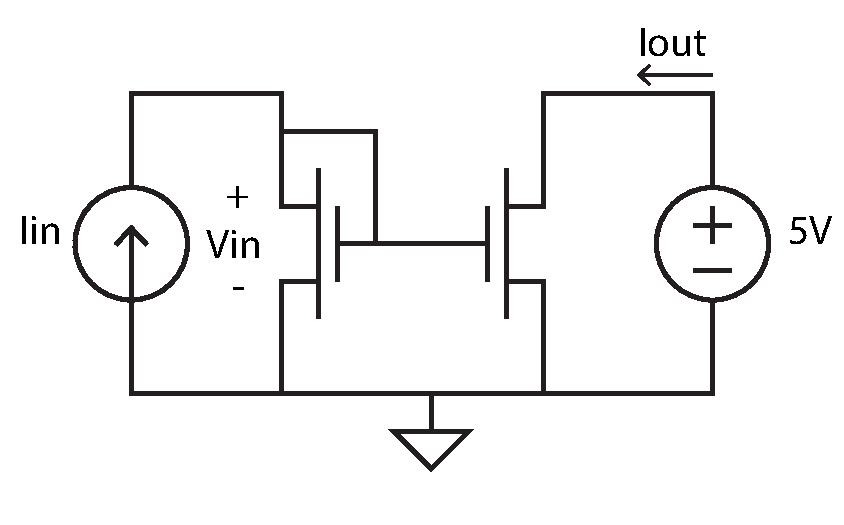
\includegraphics[width=0.6\linewidth]{../diagrams/lab4_exp2_circuit.pdf}
   		\caption{The schematic for the experimental setups used in Experiment 2. Two of four ALD1106 transistors were used.}\label{fig:exp2_diag}
	\end{figure}
	\begin{figure}[H]
 		\centering
   		
\includegraphics[width=0.6\linewidth]{../diagrams/lab4_exp2_plt.pdf}
   		\caption{The current transfer characteristic of the nMOS current mirror circuit in depicted in Figure \ref{fig:exp2_diag} when the current source was varied from 1nA to 1mA and the corresponding theoretical fit where $I_{out} = I_{in}$}\label{fig:exp2_plot}
	\end{figure}
	\subsection{Analysis}
	The error of the current mirror circuit was calculated as $\frac{100}{1000}\sum \frac{|I_{out} - I_{in}|}{I_{in}}$. The error was found to be 11.219\%. This error is likely due to the fact the current source is not ideal and there may have been some error in the measurement as well as some variation in the transistors used in the circuit due to manufacturing defects. 
	\subsection{Discussion}
	The error is still relatively low and this circuit is able to approximate the behavior of an ideal current mirror. The behavior of the current mirror is consistent with the theoretical fit, especially for higher currents. The error is likely more significant at lower currents due to the fact that the current source may not be able to provide a stable current at such low levels and there may be more noise in the measurements. Overall, this circuit is a good approximation of an ideal current mirror and can be used in various applications where a stable current source is needed.
\section{Output/Drain Characteristics}
	\subsection{Results}
	\begin{figure}[H]
 		\centering
   		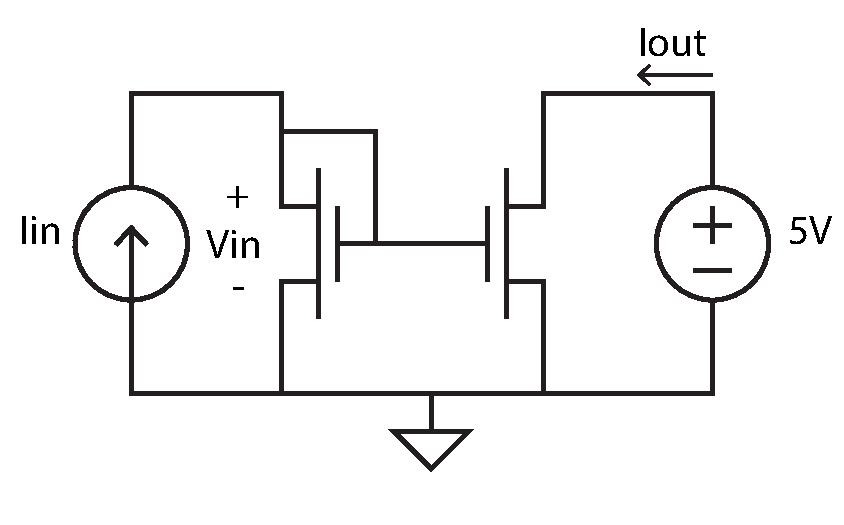
\includegraphics[width=0.6\linewidth]{../diagrams/lab4_exp3_circuit.pdf}
   		\caption{The schematic for the experimental setups used in Experiment 3. Two of four ALD1106 transistors were used.}\label{fig:exp3_diag}
	\end{figure}

	\begin{figure}[H]
 		\centering
   		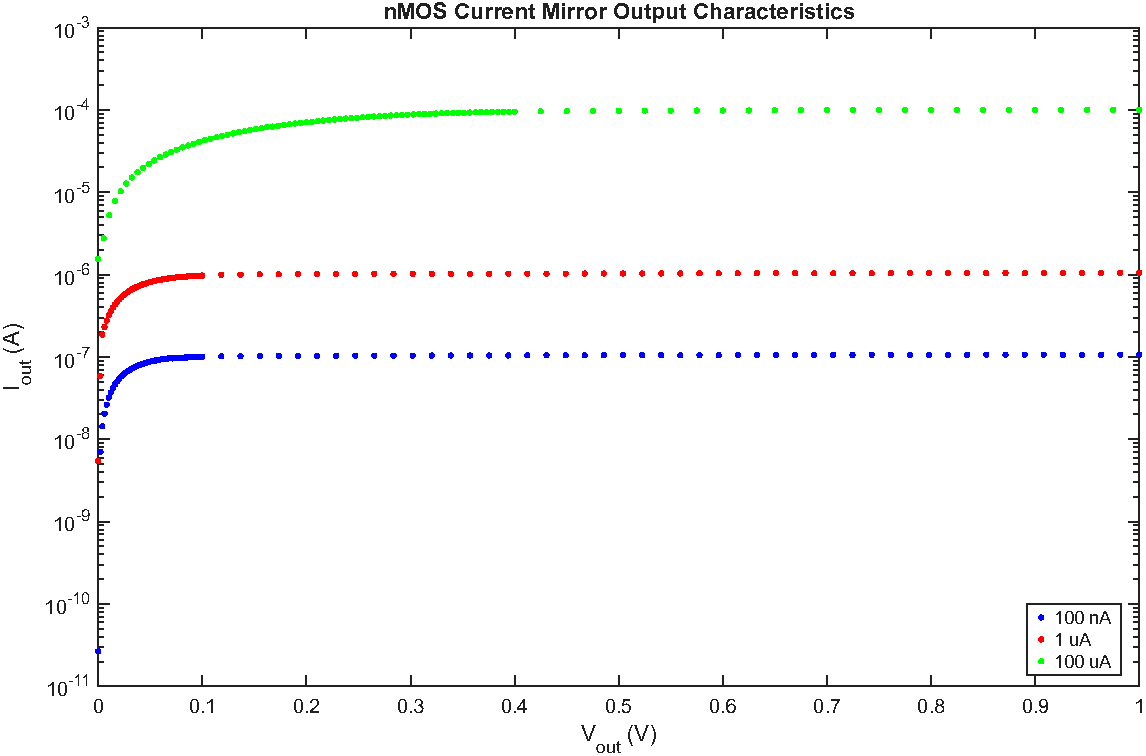
\includegraphics[width=0.6\linewidth]{../diagrams/lab4_exp3_plot.pdf}
   		\caption{Semilog plot of the nMOS current mirror output characteristics ($I_{out}$ vs.\ $V_{out}$) for input currents of 100 nA, 1 $\mu$A, and 100 $\mu$.}\label{fig:exp3_plot1}
	\end{figure}
	
	\begin{table}[h]
		\centering
		\begin{tabular}{c c c c c}
			\toprule
			$I_\mathrm{in}$ (A) & $r_\mathrm{on}$ ($\Omega$) & $r_\mathrm{o}$ ($\Omega$) & $V_\mathrm{A}$ (V) & Gain \\
			\midrule
			$1\times10^{-7}$  & $3.653\times10^{5}$ & $3.208\times10^{8}$ & 32.081 & 878.3 \\
			$1\times10^{-6}$  & $4.069\times10^{4}$  & $3.002\times10^{7}$ & 30.019 & 737.8 \\
			$1\times10^{-4}$  & $2.532\times10^{3}$  & $2.683\times10^{5}$ & 26.829 & 106.0 \\
			\bottomrule
		\end{tabular}
		\caption{Extracted nMOS current mirror parameters for different input currents using corrected region selection and absolute current fitting.}
		\label{tab:nmos_parameters}
	\end{table}
	\subsection{Analysis}
	From the measured output characteristics, we got the on-resistance ($r_\mathrm{on}$) from the slope of the output current in the deep ohmic region and the output resistance ($r_\mathrm{o}$) from the slope in the saturated region. 
	The Early voltage ($V_\mathrm{A}$) was calculated as $V_\mathrm{A} = r_\mathrm{o} I_\mathrm{in}$, and the intrinsic gain was calculated as $\mathrm{Gain} = r_\mathrm{o}/r_\mathrm{on}$. \\\\
	As expected, the on-resistance decreases with increasing input current. This reflects the transition from weak inversion (high $r_\mathrm{on}$) to strong inversion (low $r_\mathrm{on}$). The output resistance also decreases with increasing current due to stronger channel-length modulation effects at higher currents. 
	The Early voltage shows a similar trend, slightly decreasing with increasing input current. The intrinsic gain is highest in weak inversion, slightly lower in moderate inversion, and drops significantly in strong inversion.

	\subsection{Discussion}
	The assumption that the intrinsic gain of the transistor is much greater than unity is generally valid in weak and moderate inversion, where gains are 878 and 738, respectively. In strong inversion, the gain drops to approximately 106, which is still larger than unity but significantly lower, indicating that some approximations based on very large gain might be less accurate. \\\\
	Overall, the measurements confirm that the transistor behaves nearly ideally in weak and moderate inversion, with relatively flat saturation characteristics and high intrinsic gain. The strong inversion regime shows more pronounced channel-length modulation, reflected in the lower gain and Early voltage. These results are consistent with the expected trends for MOSFET current mirrors.
%----------------------------------------------------------

\end{document}